\thispagestyle{empty}
{\Huge\forallx} %modify \forallx command in style file under TITLE AND VERSION DATA 

{\tt An Introduction to Formal Logic\\
this copy compiled \today}
\vfill



% {\sf Benjamin Brast-McKie}\\
% \emph{Massachusetts Institute of Technology}
% \\
{\sf Jonathan Jenkins Ichikawa}\\
\emph{University of British Columbia}
\\
{\sf P.D.\ Magnus}\\
\emph{University at Albany, State University of New York}\\




{\sf With sections lifted from the Calgary Remix by Magnus, Button, Loftis, Trueman, Thomas-Bolduc, and Zach}\\
%\emph{Calgary Remix Gang}\\

{\sf Adapted for MIT by Josh Hunt and Benjamin Brast-McKie}\\




\vfill




{\sf
	MIT 24.241 Fall 2023 edition \\%version 2.2 [\bookversion]\\
	source material: fecundity.com/logic, v1.30\\
	This book is offered under a Creative Commons license.\\
	(Attribution-ShareAlike 3.0)
}



\newpage
\thispagestyle{empty}%

\iffalse
\begin{figure}[h!]
  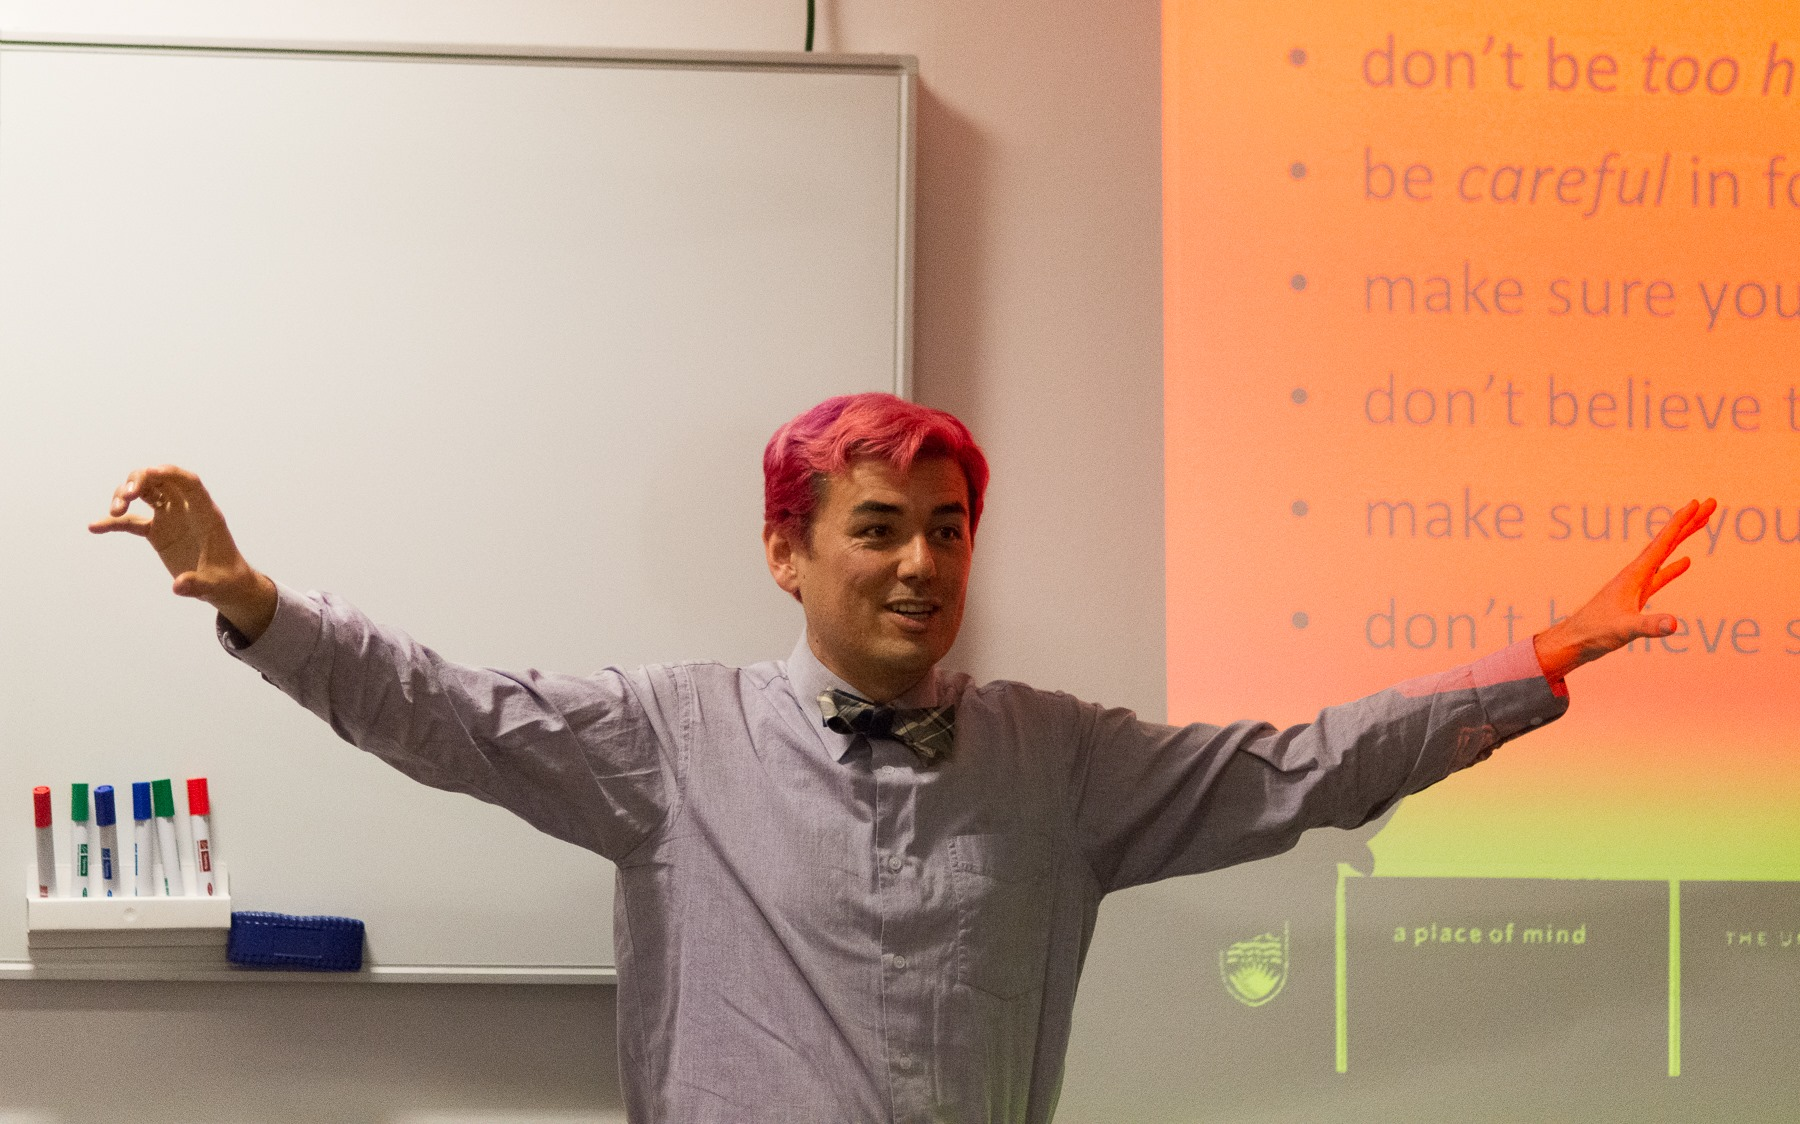
\includegraphics[width=\linewidth]{images/ichikawa.jpg}
  \centering
\end{figure}
\fi

{\sf
Jonathan Ichikawa, who modified the Magnus edition to create this version, would, first and foremost, like to thank P.D.\ Magnus. He is also grateful to Greg Restall, and his book \emph{Logic}, which is the first text he taught from and which is the model for the discussion of trees. He also thanks the many UBC students who test-drove drafts of the book. He's also grateful for helpful conversations with Roberta Ballarin, Roy Cook, Josh Dever, Dave Gilbert, Thony Gillies, and Jon Shaheen.

The original author, P.D.\ Magnus, would like to thank the people who made this project possible. Notable among these are Cristyn Magnus, who read many early drafts; Aaron Schiller, who was an early adopter and provided considerable, helpful feedback; {and} Bin Kang, Craig Erb, Nathan Carter, Wes McMichael, Selva Samuel, Dave Krueger, Brandon Lee, Toan Tran, and the students of Introduction to Logic, who detected various errors in previous versions of the book.
}

\vfill
{
\copyright\ \ifthenelse{\year=2005}{\number\year}{2005--\number\year} by P.D. Magnus and Jonathan Ichikawa. Some rights reserved.
}

{\footnotesize
You are free to copy this book, to distribute it, to display it, and to make derivative works, under the following conditions: (a) Attribution. You must give the original author credit. (b) Share Alike. If you alter, transform, or build upon this work, you may distribute the resulting work only under a license identical to this one. --- For any reuse or distribution, you must make clear to others the license terms of this work. Any of these conditions can be waived if you get permission from the copyright holder. Your fair use and other rights are in no way affected by the above. --- This is a human-readable summary of the full license, which is available on-line at \url{http://creativecommons.org/licenses/by-sa/3.0/}

Typesetting was carried out  in \LaTeX$2\varepsilon$. The style for natural deduction proofs is based on fitch.sty (v0.4) by Peter Selinger. Tree typesetting from prooftrees (v0.6) by Clea F. Rees. This copy of \forallx\ is current as of \today.
}
